\section{Event Patterns} \label{EventPatters}
This section will present a statemachine diagram for each class. Each statemachine diagram is the result of examining each class, with a focus on identifying the different states of the class' objects and the events which effects the objects and changes their state. An event can happen without changing the state of the class e.g. on \cref{MealClass} the \textit{Change scale} event will not lead to a new state for the meal class object.  

Each class examination starts, by showing a few of the event patterns that was formulated for the specific class. The relationship between the classes and events are described in \cref{tab:EventTable}. The event patterns will then be used to model the statemachine diagram for the specific class. The event patterns and statemachine diagrams are created to get a better understanding of the dynamic in the problem domain. It is possible to use the event definitions in \cref{EventsSection} for a better understanding of each event the event behaviour is not clear from the event name.   

\subsection{Food Class}
Some of the event patterns used to understand the behavior of this class are:
\begin{itemize}
	\item Added -> Expired -> Quantity changed -> Removed.
	\item Added -> Quantity changed -> Expired -> Quantity changed -> Unexpired -> Removed.
	\item Shopping list item added -> Added -> Expired -> Removed.
	\item Shopping list item added -> Shopping list item removed.
\end{itemize}

This class also has some event patterns which are not legal e.g. 
Shopping list item added -> Expired.

\begin{figure}[tbhp]
	\centering
	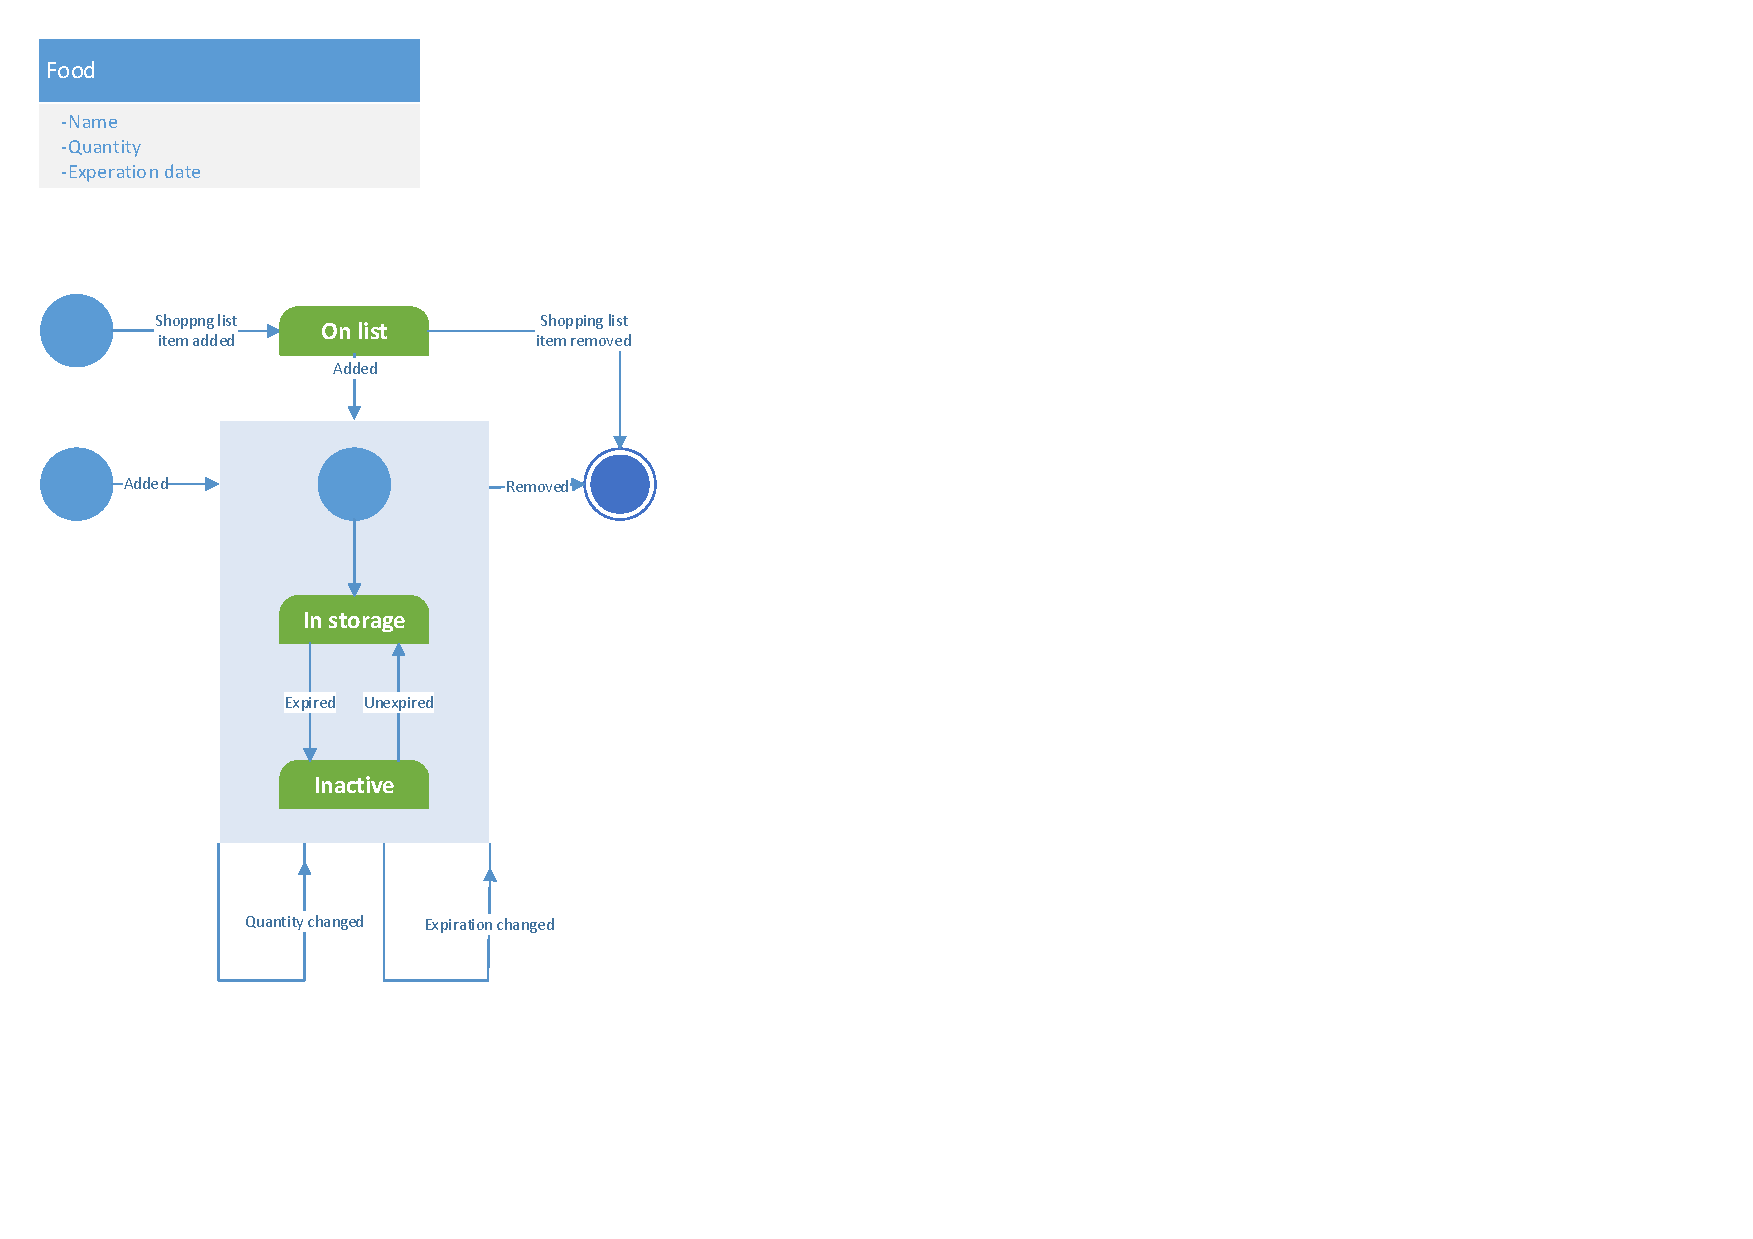
\includegraphics[clip=true, trim=0.5cm 4cm 18.5cm 0.5cm,  ]{Development/ProblemDomain/FoodClass.pdf}
	\caption{Statemachine diagram for the food class} \label{FoodClass}
\end{figure}
The \cref{FoodClass} is described with a focus on the flow of the diagram.
An object of this class can be instantiated when the user either adds a shopping list item or adds a food item directly to their inventory. The two starting events for this class are therefore \textit{Shopping list item added} and \textit{Added}. The two start events sets the object's state to either \textit{On list} or \textit{In storage}. The On list state can be changed by the Add event, which sets the state to In storage, or by the \textit{Shopping list item removed} event, which terminates the object. The object can also have the state \textit{Inactive}. This state can be set by the expired \textit{Expired} event and reset to In storage by the \textit{Unexpired} event. It is possible for an object in both the In storage state and Inactive state to be effected by the \textit{Quantity changed} event and \textit{Expiration changed} event without changing the object's state. These two events can be iterated throughout an object's lifetime. The object can also be terminated from the In storage and Inactive state, by the \textit{Removed} event.   

\subsection{Meal Class}
Some of the event patterns used to understand this class are:
\begin{itemize}
	\item Meal added -> Change scale -> Meal prepared.
	\item Meal added -> Change date -> Meal prepared.
	\item Meal added -> Day passed -> Reschedule meal -> Meal prepared.
	\item Meal added -> Change scale -> Change date -> Change scale -> Meal prepared.
\end{itemize}

An example of event patterns that are not legal for this class are: Meal added -> Day passed -> Change Scale.

\begin{figure}[H]
	\centering
	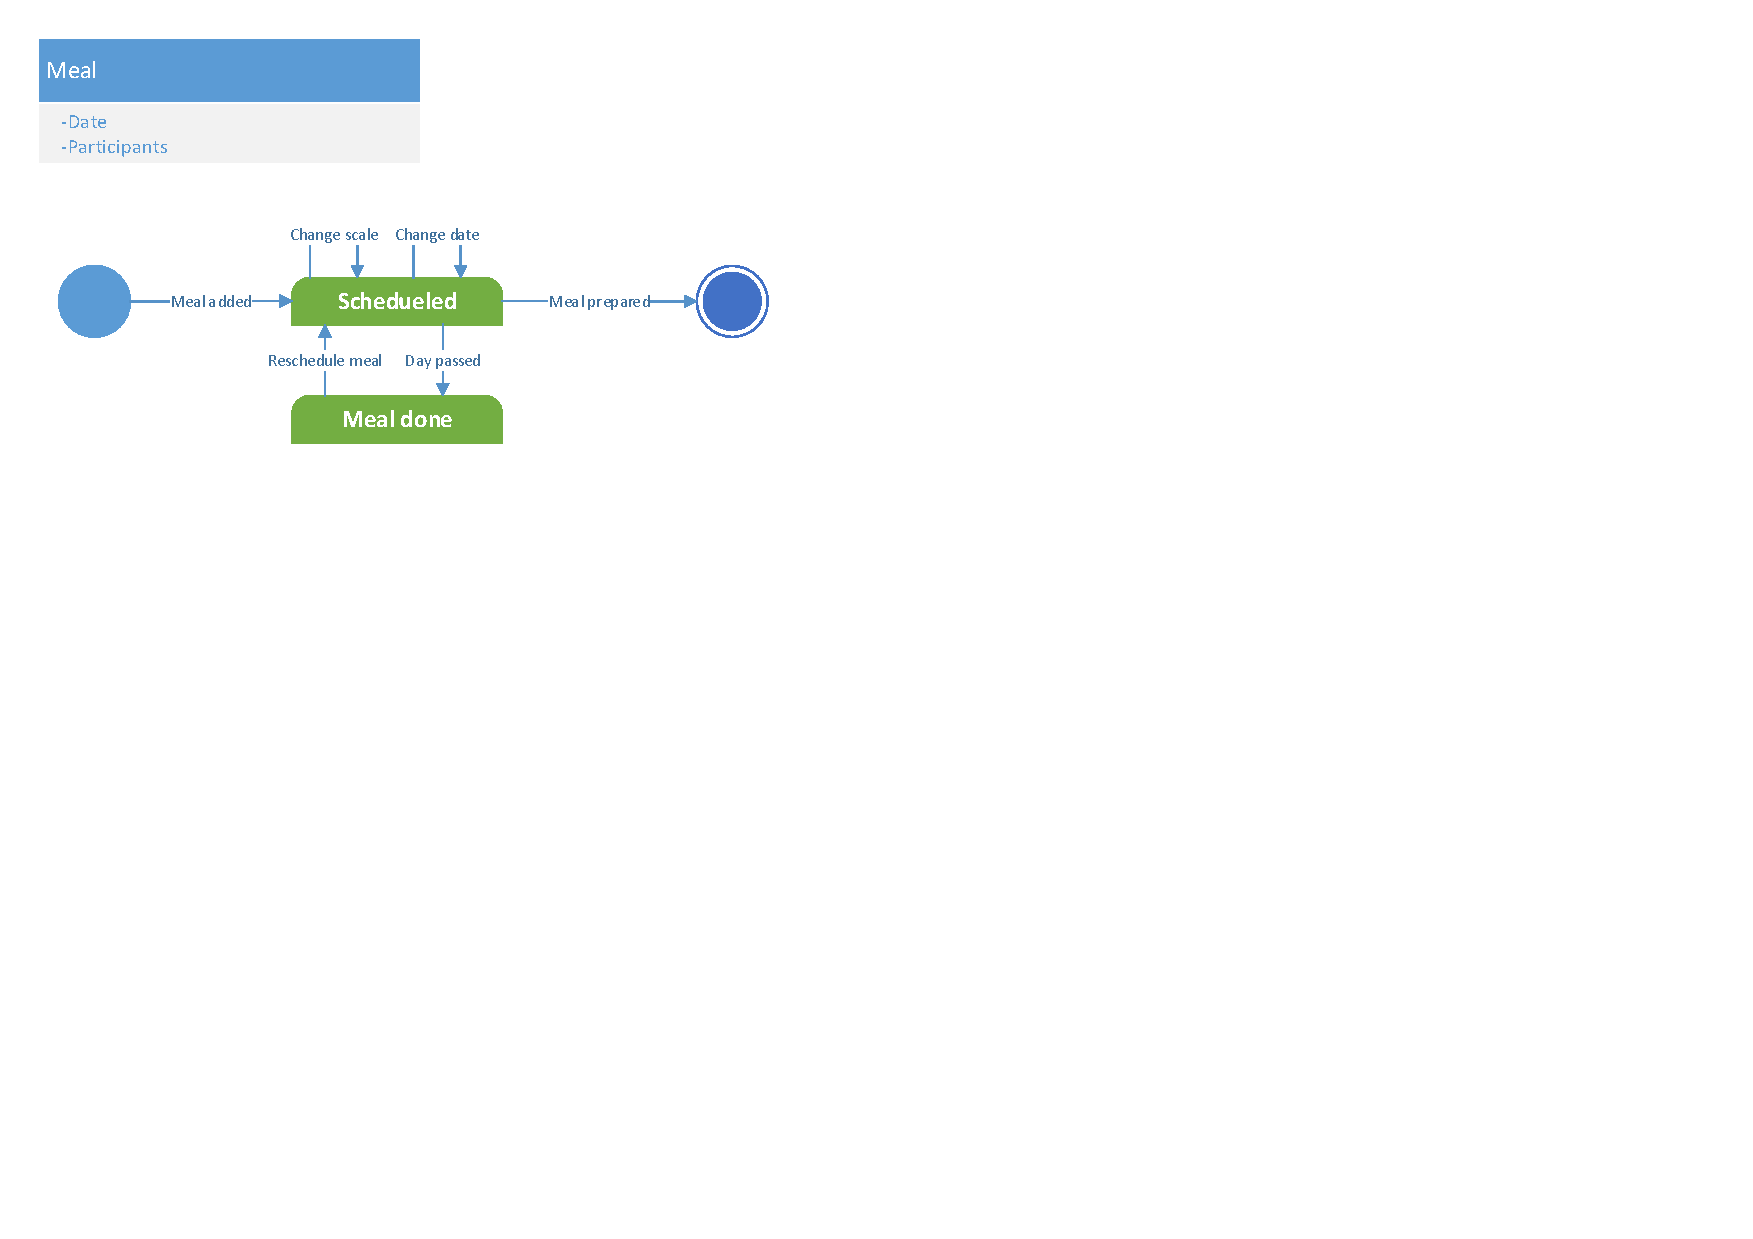
\includegraphics[clip=true, trim=0.5cm 13cm 16.5cm 0.5cm]{Development/ProblemDomain/MealClass.pdf}
	\caption{Statemachine diagram for the meal class} \label{MealClass}
\end{figure}

An object of the meal class can be instantiated by the \textit{Meal added} event. This sets the state of the object to \textit{Scheduled}. The events \textit{Change scale} and \textit{Change date} can be iterated throughout the object's lifetime and does not change the state of the object. The object can also have the \textit{Meal done} state, which can be set by the \textit{Day passed} event and reset to Scheduled by the \textit{Reschedule meal} event. The object can only be terminated by the \textit{Meal prepared} event.

\subsection{User Settings Class}

\begin{figure}[H]
	\centering
	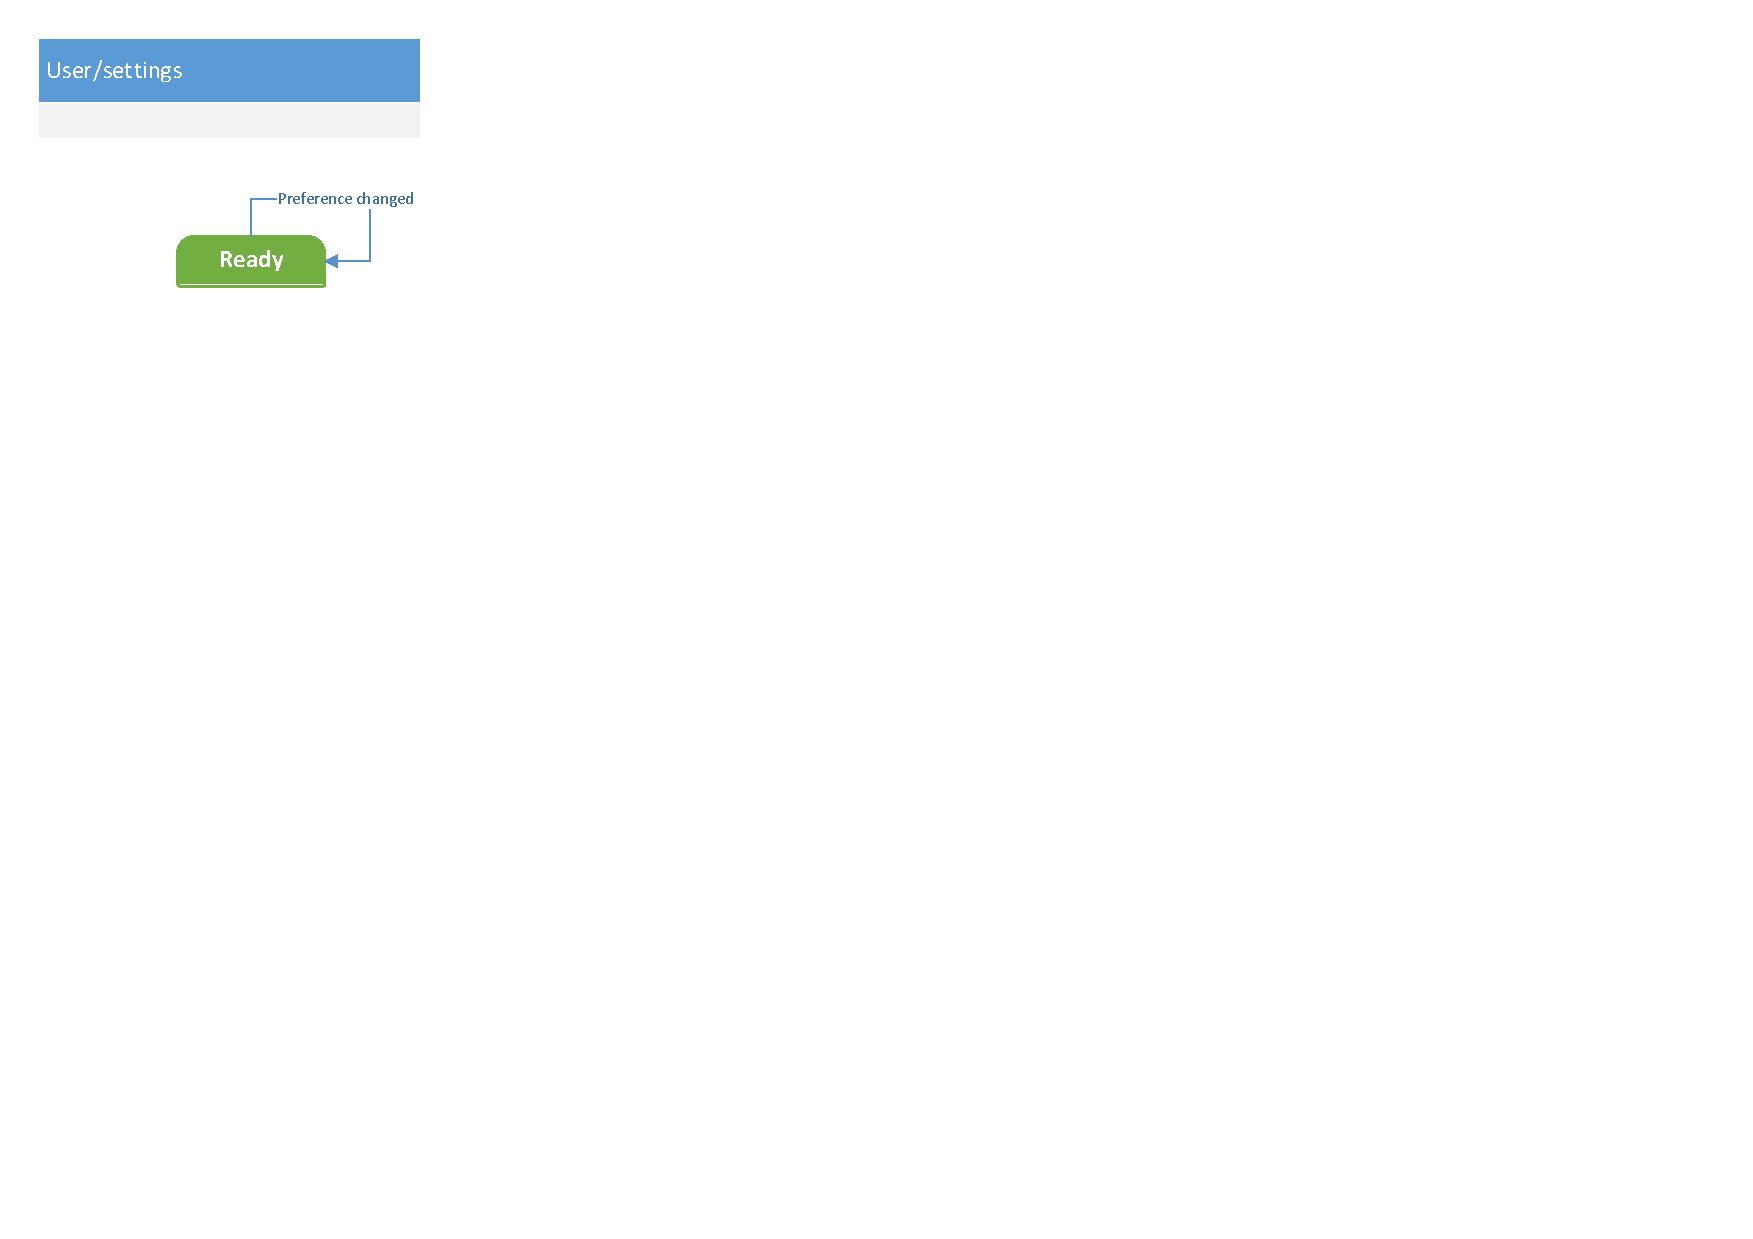
\includegraphics[clip=true, trim=0.5cm 15.5cm 22.5cm 0.5cm]{Development/ProblemDomain/UserSettingsClass.pdf}
	\caption{Statemachine diagram for the user settings class} \label{UserSettingsClass}
\end{figure}
The \textbf{User settings} class contains preferences from the user which the system should take into consideration.

\subsection{Recipe Class}
Some of the event patterns used to understand this class are:
\begin{itemize}
	\item Recipe added -> Recipe removed.
	\item Recipe added -> Recipe found -> Meal added -> Meal Removed.
	\item Recipe added -> Recipe found -> Recipe found -> Meal added -> Meal Removed.
\end{itemize}

One of the event patterns which are not legal for this class are: Recipe added -> Recipe found - Meal removed.

\begin{figure}[H]
	\centering
	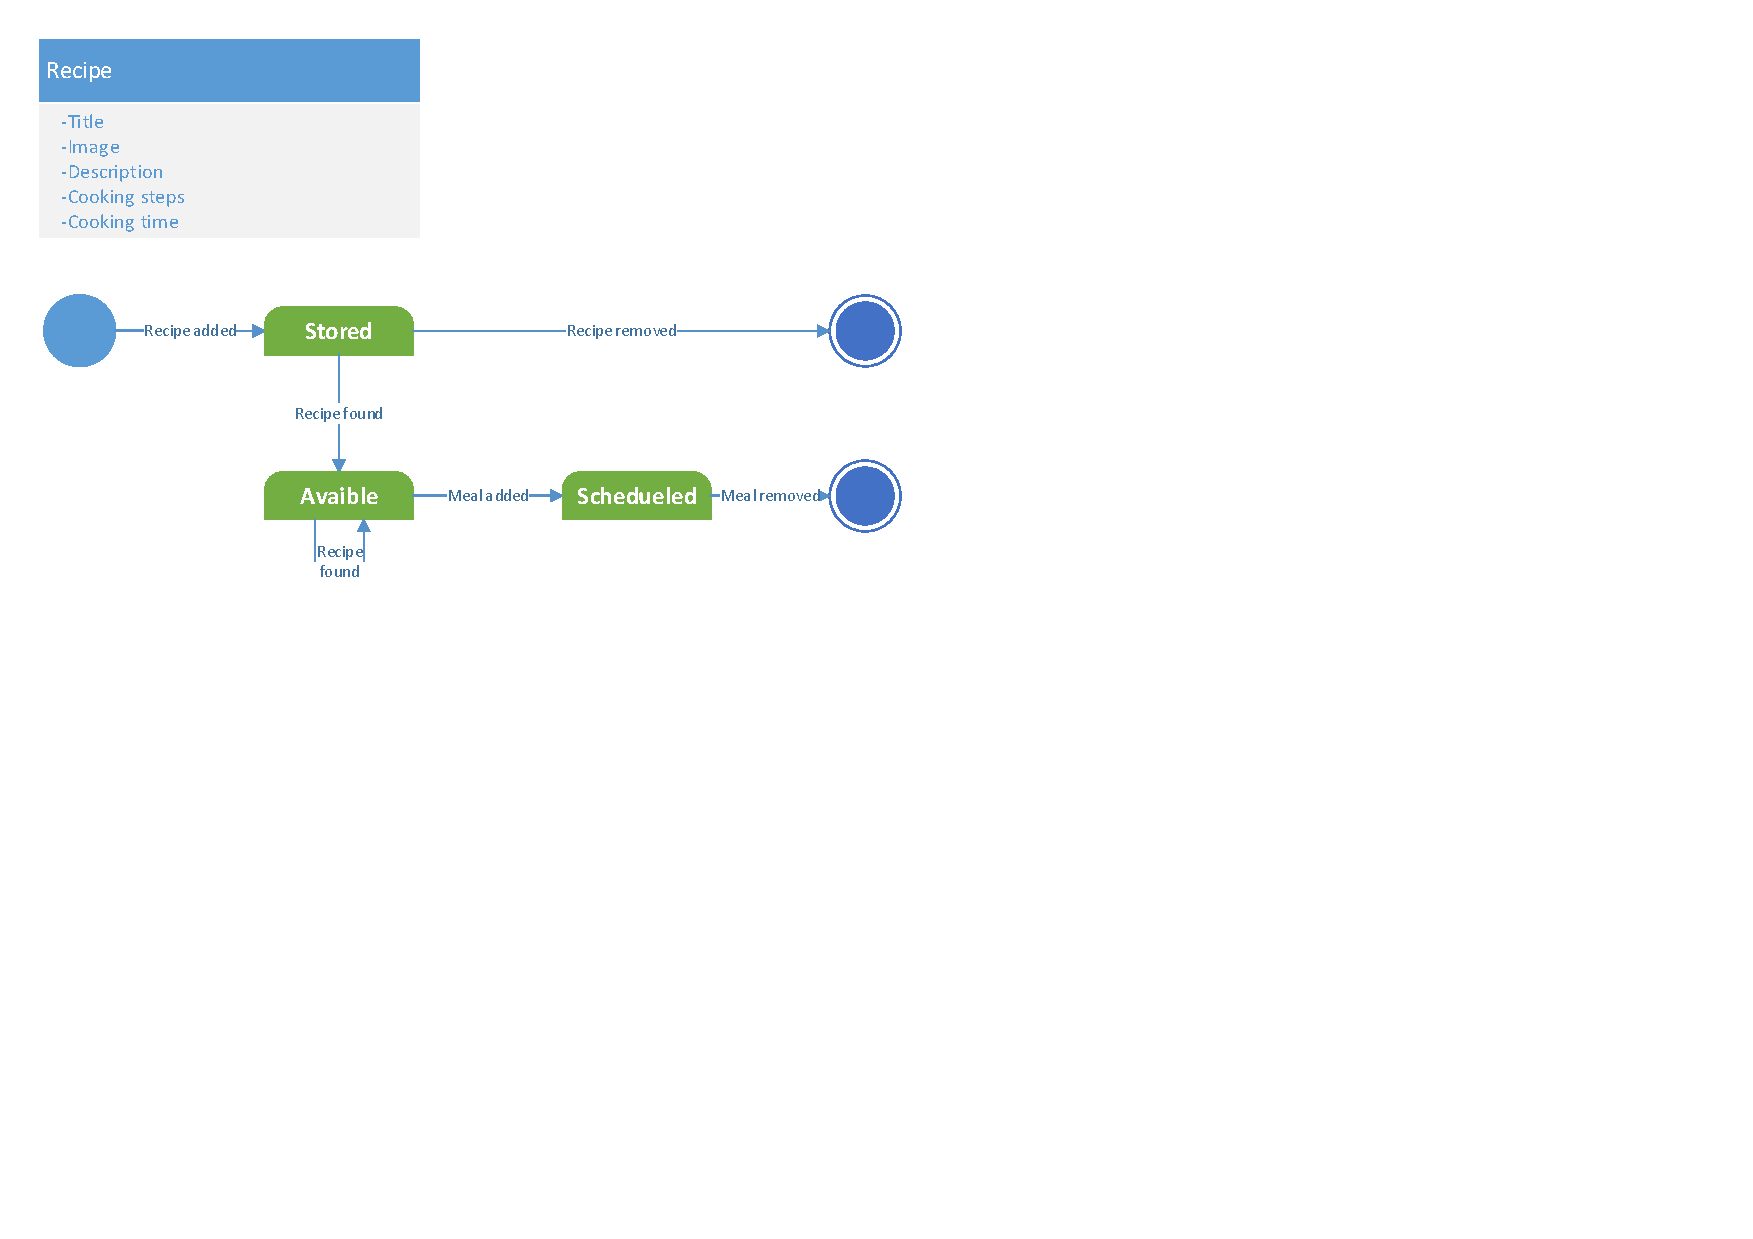
\includegraphics[clip=true, trim=0.5cm 11cm 14cm 0.5cm]{Development/ProblemDomain/RecipeClass.pdf}
	\caption{Statemachine diagram for the recipe class} \label{RecipeClass}
\end{figure}

An object of the Recipe class can only be instantiated by the \textit{Recipe added} event. This event sets the state of the object to \textit{Stored}. From this state the \textit{Recipe removed} event can terminate the object. The \textit{Recipe found} event can change the object's state from Stored to \textit{Available}. The same event can also be iterated in this state, without changing the state. the \textit{Meal added} event can change the objects state to \textit{Scheduled}. From this state the \textit{Meal removed} event can terminate the object.